\documentclass[conference]{IEEEtran}
\IEEEoverridecommandlockouts
\usepackage{cite}
\usepackage{amsmath,amssymb}
\usepackage{graphicx}
\usepackage{booktabs}
\usepackage{multirow}
\usepackage{xcolor}
\usepackage[hidelinks]{hyperref}
\graphicspath{{figures/}}

% Numbers in this paper come from results/*.csv and results/diagnostics/history_diagnostics.csv
% (config 87f5489e9d59; seeds split 2026, bootstrap 20260914). Brackets are 95% group-bootstrap CIs.

\begin{document}

\title{Same Score, Different Story: How Resampling History Shapes What Spatial--Frequency Features Detect in AI-Generated Images}

\author{\IEEEauthorblockN{Member One, Member Two, Member Three}
\IEEEauthorblockA{Department of Computer Science and Engineering\\
United International University, Dhaka, Bangladesh\\
CSE 4883: Digital Image Processing, Summer 2026}}

\maketitle

\begin{abstract}
Simple pixel and frequency statistics are popular, interpretable cues for telling AI-generated images from photographs, yet public datasets differ between the two classes in processing history: file format, image size, and prior compression. We compare three simple feature sets, seven pixel-pattern statistics, seven frequency statistics, and their combination, under a pipeline fixed before any data was processed, with identical processing for both classes, splits by image group, one logistic-regression classifier, and group-bootstrap confidence intervals. On 3,000 GenImage images (BigGAN, Stable Diffusion v1.4, ADM), the combined set gives the highest pooled AUROC (0.793 [0.759, 0.826]). Matched JPEG compression changes pooled AUROC by at most 0.027, and holding Stable Diffusion v1.4 out of training lowers its AUROC by 0.078 [0.034, 0.124], to 0.629 [0.571, 0.690] at JPEG quality 75. Per-generator analysis shows what the pooled score hides: the pipeline's own 2$\times$ upsampling of BigGAN lets high-frequency features separate it almost perfectly. A one-step diagnostic that gives every image the same resampling history leaves pooled AUROC unchanged (0.796 vs.\ 0.802) but moves per-generator AUROC by $-0.17$ to $+0.30$, removes the frequency arm's advantage over the pixel arm, and lifts the pixel arm on the unseen generator from chance (0.477) to 0.771. For simple features, which generator is ``easy'' and which feature family ``wins'' depends on resampling history, and pooled AUROC cannot show it.
\end{abstract}

\begin{IEEEkeywords}
AI-generated image detection, image forensics, frequency analysis, JPEG compression, dataset bias, resampling
\end{IEEEkeywords}

\section{Introduction}

Image generators now produce pictures that look natural at a glance, and detecting them is a practical image-forensics problem. Beside learned detectors, simple statistics remain popular because they are cheap and explainable: spectral band energies, the spectral slope, and spectral peaks trace back to generator upsampling~\cite{frank2020leveraging,dzanic2020fourier,durall2020watch,zhang2019artifacts}, and local pixel statistics such as gradients and high-pass residuals carry related signal~\cite{nataraj2019cooccurrence,tan2024npr}.

These cues are usually evaluated on public datasets in which the two classes arrive differently. In GenImage~\cite{zhu2023genimage}, every real photograph is an ImageNet JPEG of varying size, while every generated image is a fixed-size PNG: 128\,px for BigGAN, 256\,px for ADM, and 512\,px for Stable Diffusion v1.4. Grommelt et al.~\cite{grommelt2024fake} and B-Free~\cite{guillaro2025bfree} showed that detectors exploit such format and size differences. Any pipeline that brings images to one size must resample them, and it resamples each class by a different factor. The published evidence on this bias is at the detector level; it does not say which individual statistics are affected, or how the verdict ``which feature family works best'' depends on it.

We study the question at the level of explainable features. With identical processing for both classes and a strict split by image group, which simple feature set separates real from generated images best, and how does the answer change under matched JPEG compression and on a generator never seen in training? We answer it with a pipeline fixed in advance (Fig.~\ref{fig:pipeline}) and then add one diagnostic that changes only how images are resampled.

\textbf{Contributions and novelty.} (i) A leakage-controlled, per-feature and per-generator comparison of pixel, frequency, and combined features under matched JPEG and an unseen generator, with paired group-bootstrap intervals. (ii) Evidence that the pooled AUROC hides processing history: file facts alone classify the dataset perfectly, and the strongest ``frequency evidence'' is a resampling artifact created by the pipeline itself. (iii) A resampling-matched diagnostic in which the BigGAN images are pixel-identical to the original pipeline, so every change in BigGAN separation comes from the real images' processing alone. It shows that pooled AUROC stays the same while per-generator results and the ranking of the feature families change. Zhou and Wang~\cite{zhou2026fragile} recently reported that resize versus native-resolution preprocessing flips per-generator conclusions for training-free detectors. We are not aware of work that measures this effect for individual explainable statistics, combines it with matched JPEG and an unseen-generator test, and isolates the resampling mechanism with identical fakes.

\section{Related Work}

\textbf{Dataset bias.} Grommelt et al.~\cite{grommelt2024fake} showed that JPEG and size differences in GenImage can look like detection evidence, and that matching them changes cross-generator results. B-Free~\cite{guillaro2025bfree} removed content, format, and size differences from training and showed that leading detectors rely on them. SFLD~\cite{gye2025sfld} quantified content bias, and Chameleon~\cite{yan2025sanity} showed that easy data overstates detectors. Zhou and Wang~\cite{zhou2026fragile} audited training-free detectors and found preprocessing and compression choices change per-generator conclusions. These studies work at the detector level; we work at the level of fourteen named statistics.

\textbf{Frequency and pixel cues.} Spectral differences arise from generator upsampling~\cite{frank2020leveraging,durall2020watch,zhang2019artifacts} and concentrate in the high band~\cite{dzanic2020fourier}. Dong et al.~\cite{dong2022think} showed that such traces can be weakened, and Sato et al.~\cite{sato2026radial} classify with radial spectrum templates built from real images. Co-occurrence~\cite{nataraj2019cooccurrence} and neighbouring-pixel relations~\cite{tan2024npr} are the pixel-level counterparts.

\textbf{Generator shift.} Wang et al.~\cite{wang2020cnn} tested JPEG and unseen generators together; Corvi et al.~\cite{corvi2023detection} measured the drop from GAN-era detectors to diffusion images; GenImage~\cite{zhu2023genimage} and AI-GenBench~\cite{pellegrini2025aigenbench} make unseen-generator testing standard. Following UniversalFakeDetect~\cite{ojha2023universal}, we use fixed features with one simple classifier, so that differences between arms reflect the features. Reconstruction-based detectors~\cite{wang2023dire,ricker2024aeroblade,chu2025fire} need generator access and are outside our scope.

\section{Method}

\begin{figure}[t]
\centering
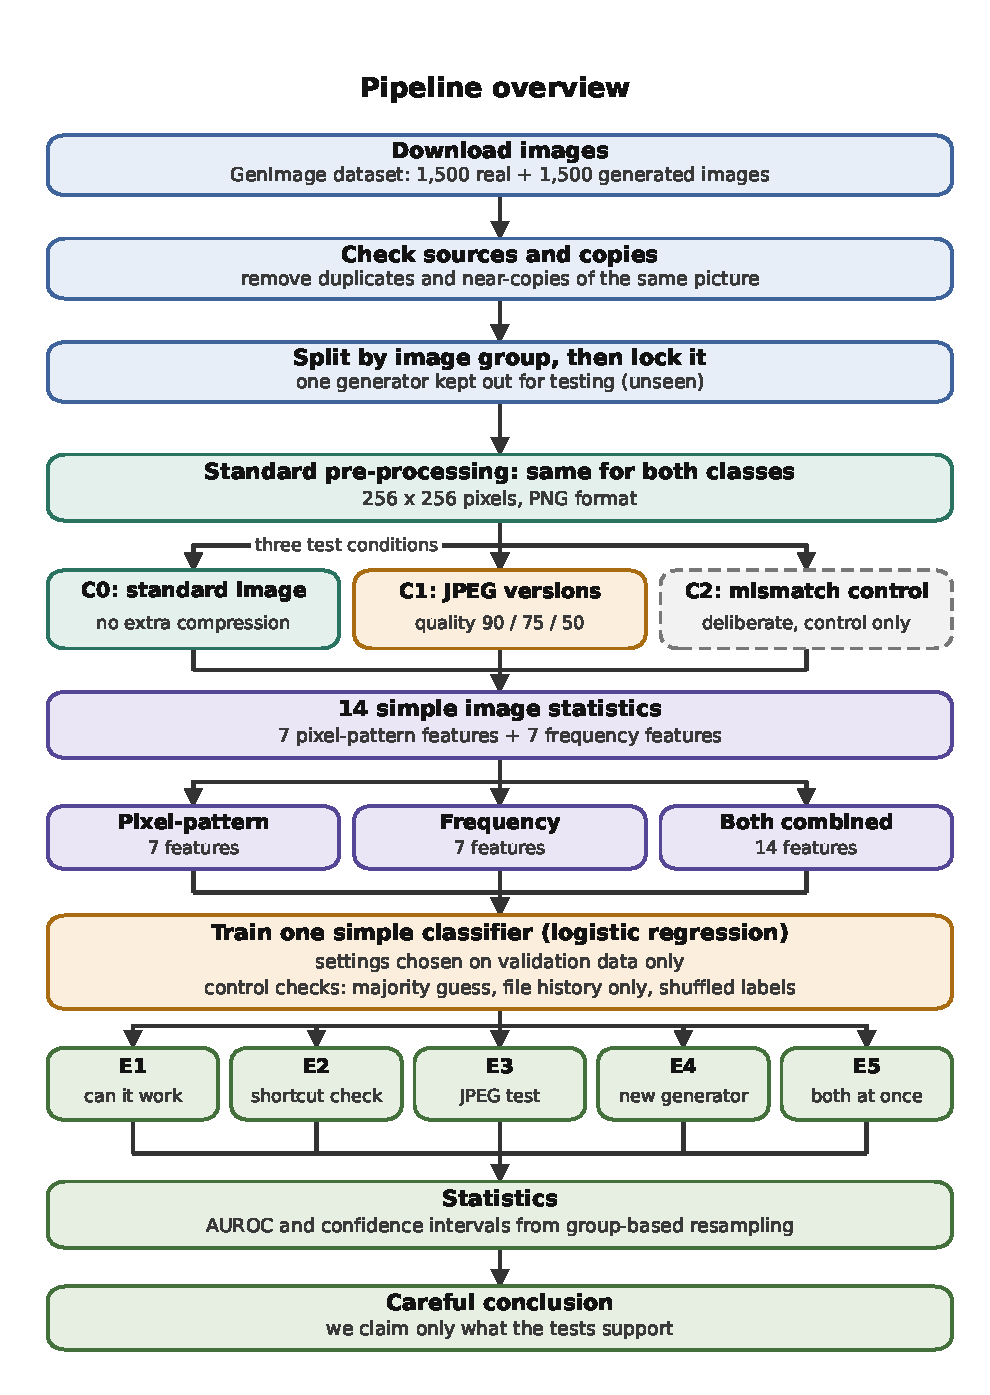
\includegraphics[width=0.84\columnwidth]{pipeline-diagram.pdf}
\caption{The pipeline, fixed before any image was processed. Every stage runs automatic checks and stops the study on a failure.}
\label{fig:pipeline}
\end{figure}

\subsection{Data and integrity checks}
We stream the validation folders of three GenImage subsets (BigGAN, SD v1.4, ADM) from a public mirror, keep images by a content-blind hash of the file path, and draw 500 real and 500 generated images per subset with a fixed seed: 3,000 parent images in total. Before splitting, we remove exact copies, pixel-level copies, and near-copies (64-bit DCT perceptual hash, Hamming distance $\le 4$), images with non-sRGB colour profiles (about 10\% of the ImageNet reals), and images with real transparency. The original file facts of every image (format, width, height) are recorded.

\subsection{Conditions}
\textbf{C0} (canonical): shorter side resized to 256\,px with bicubic interpolation, centre crop to $256\times256$, lossless PNG, identical for both classes. The resize factor this implies differs by class: $2.0$ for BigGAN, $1.0$ for ADM, $0.5$ for SD v1.4, and a median of $0.68$ for reals. \textbf{C1}: both classes re-encoded from C0 as JPEG at quality 90, 75, and 50 (Pillow, 4:2:0). \textbf{C2}: a deliberate mismatch control (reals JPEG~75, fakes PNG).

\textbf{R} (resampling-matched diagnostic, added after the study concluded): every image is centre-cropped to $128\times128$ at its native resolution, with no resampling, and then upsampled $2\times$ bicubic to $256\times256$. All images now share one resampling operation. Because BigGAN images are $128\times128$, their R images are pixel-identical to their C0 images (checked in code), so any change in BigGAN separation comes from the reals. For the other classes, R also narrows the field of view (a 128\,px crop spans 25\% of an SD image's side and about a third of a typical real's shorter side). Six reals smaller than 128\,px are dropped, leaving 599 of the 600 test parents.

\subsection{Features}
Fourteen features are computed on luminance in $[0,1]$. \textit{Pixel arm (f01--f07):} intensity variance, skewness, excess kurtosis, Sobel gradient-magnitude mean and standard deviation, Laplacian variance, and the variance of the residual after a $3\times3$ binomial blur. \textit{Frequency arm (f08--f14)}, from the Hann-windowed power spectrum after mean removal: energy fractions in the low (0--0.05), mid (0.05--0.25), and high (0.25--0.5 cycles/pixel) bands; the Nyquist ratio of top-band (0.375--0.5) to high-band energy; the log--log radial spectral slope; the coefficient of variation of mid-band energy over twelve $30^\circ$ sectors; and the largest non-DC local maximum over total non-DC power. Every definition was fixed and checked against hand calculations on synthetic images (constant, impulse, edge, checkerboard, sinusoid, $1/f$ noise) before real data was touched.

\subsection{Classifier, splits, and statistics}
One L2 logistic regression with balanced class weights serves all three arms; the standardiser is fitted on training data, the regularisation strength $C\in\{0.01,0.1,1,10\}$ is chosen by validation AUROC, and the threshold by validation balanced accuracy. The split is 60/20/20 by parent image group. One locked test set of 600 parents (300 real, 100 per generator) is shared by all experiments, so every comparison between experiments is paired on the same images. In the unseen-generator fold, all SD v1.4 fakes are removed from training and validation. AUROC (generated as the positive class) is the primary metric, with 95\% confidence intervals from 1,000 rounds of bootstrap over test parents. Per-generator AUROC compares one generator's test fakes against all 300 test reals.

\subsection{Experiments and controls}
Table~\ref{tab:exp} lists the experiments. Every experiment runs four controls: an always-guess classifier; a classifier on the analysed files' format and size; training on shuffled labels (mean over 200 shuffles; changed from a single shuffle after the first run stopped on it, with the diagnosis and change recorded before the rerun); and a classifier on the \emph{original} file facts before processing.

\begin{table}[t]
\centering
\caption{Experiments. E1--E5 were fixed in advance; R is a post-hoc diagnostic.}
\label{tab:exp}
\footnotesize
\setlength{\tabcolsep}{2.5pt}
\resizebox{\columnwidth}{!}{%
\begin{tabular}{@{}llll@{}}
\toprule
ID & Question & Condition & Training generators \\
\midrule
E1 & Does any arm separate the classes? & C0 & all three \\
E2 & Does a deliberate mismatch help? (control) & C2 & all three \\
E3 & What does matched JPEG change? & C1 (q90/75/50) & all three \\
E4 & Does it transfer to a new generator? & C0 & SD v1.4 held out \\
E5 & Unseen generator + JPEG together & C1 (q75) & SD v1.4 held out \\
R  & Does resampling history drive the result? & R & as E1 and E4 \\
\bottomrule
\end{tabular}}
\end{table}

\section{Results}

\subsection{The accepted pipeline}
Table~\ref{tab:main} summarises E1--E5. The combined arm has the highest pooled AUROC in every experiment, and every arm separates the classes in E1 (all intervals exclude 0.5). Frequency beats pixel by 0.087 [0.046, 0.130], and combined beats frequency by 0.041 [0.018, 0.064]. The per-generator columns show that the pooled number mixes very different cases: BigGAN is separated almost perfectly (frequency 0.997), whereas the two diffusion families reach 0.58--0.71.

\begin{table}[t]
\centering
\caption{Test AUROC under the accepted pipeline (C0/C1). Per-generator columns compare that generator's 100 test fakes with all 300 test reals. E5 is SD v1.4 held out, JPEG q75.}
\label{tab:main}
\footnotesize
\setlength{\tabcolsep}{2.6pt}
\begin{tabular}{@{}llcccc@{}}
\toprule
Exp. & Arm & Pooled [95\% CI] & BigGAN & SD v1.4 & ADM \\
\midrule
\multirow{3}{*}{E1} & Pixel & 0.666 [0.622, 0.707] & 0.824 & 0.581 & 0.591 \\
 & Frequency & 0.752 [0.713, 0.792] & 0.997 & 0.637 & 0.624 \\
 & Combined & \textbf{0.793} [0.759, 0.826] & 0.990 & 0.712 & 0.678 \\
\midrule
\multirow{3}{*}{E3 q50} & Pixel & 0.641 [0.596, 0.682] & 0.767 & 0.561 & 0.594 \\
 & Frequency & 0.766 [0.729, 0.806] & 0.992 & 0.632 & 0.674 \\
 & Combined & \textbf{0.794} [0.760, 0.828] & 0.974 & 0.698 & 0.709 \\
\midrule
\multirow{3}{*}{E4} & Pixel & 0.653 [0.611, 0.698] & 0.919 & 0.475$^\dagger$ & 0.566 \\
 & Frequency & 0.765 [0.726, 0.802] & 0.995 & 0.560$^\dagger$ & 0.738 \\
 & Combined & \textbf{0.789} [0.755, 0.823] & 0.984 & 0.634 & 0.749 \\
\midrule
\multirow{3}{*}{E5} & Pixel & 0.631 [0.590, 0.677] & 0.888 & 0.465$^\dagger$ & 0.540 \\
 & Frequency & 0.769 [0.730, 0.806] & 0.981 & 0.568 & 0.757 \\
 & Combined & \textbf{0.786} [0.753, 0.820] & 0.969 & \textbf{0.629} & 0.761 \\
\bottomrule
\multicolumn{6}{@{}l}{\scriptsize $^\dagger$95\% CI includes 0.5. SD v1.4 in E4/E5 is the unseen generator; E5 SD v1.4}\\
\multicolumn{6}{@{}l}{\scriptsize combined CI [0.571, 0.690].}
\end{tabular}
\end{table}

\textbf{Controls.} Always-guess scores 0.500. The analysed-file classifier scores 0.500 in C0/C1, confirming that the processed files carry no format or size cue, and 1.000 in C2, where the mismatch is real. Shuffled-label means lie between 0.503 and 0.521. The classifier on the original file facts scores 1.000 in every experiment: before processing, format and size alone separate this dataset perfectly. In E2, the content features barely use the deliberate mismatch (combined $+0.012$ [0.007, 0.017] over E1), most plausibly because the reals already carry JPEG history.

\textbf{Matched JPEG.} Refitting on compressed images changes pooled AUROC by at most 0.025 (pixel, q50). Scoring the unchanged C0 models on the compressed test images, without refitting, changes it by at most 0.027 (pixel, q50; combined $-0.019$). Compression moves the pixel arm's operating point rather than its ranking: at the threshold chosen on clean validation data, the C0 pixel model flags 98 of 300 test reals on clean images but 157 of 300 at q50 (combined: 37 to 42). At the feature level, one statistic changes meaning: the Nyquist ratio f11 separates BigGAN with univariate AUROC 0.009 at C0 but 0.772 at q50, consistent with $8\times8$ block edges adding near-Nyquist energy to images whose top band the upsampling had emptied.

\textbf{Unseen generator.} Holding SD v1.4 out lowers its AUROC by 0.078 [0.034, 0.124] (combined), 0.077 [0.026, 0.132] (frequency), and 0.106 [0.065, 0.149] (pixel), after which the pixel arm is at chance. The headline setting (E5) gives 0.629 [0.571, 0.690] for the combined arm, and adding JPEG~75 on top of the shift costs only a further 0.004.

\subsection{Where the separation comes from}
Univariate AUROCs locate the BigGAN result. At C0, five high-frequency statistics separate BigGAN from reals almost perfectly in the reversed direction (the feature is \emph{lower} for fakes): Laplacian variance 0.015, high-pass residual 0.020, high-band fraction 0.030, Nyquist ratio 0.009, and spectral slope 0.004. For SD v1.4 and ADM, all 14 features lie between 0.33 and 0.63. BigGAN is also the only class upsampled by the pipeline: bicubic $2\times$ interpolation leaves almost no energy above 0.25 cycles/pixel. The resampling-matched diagnostic tests this directly.

\begin{figure*}[t]
\centering
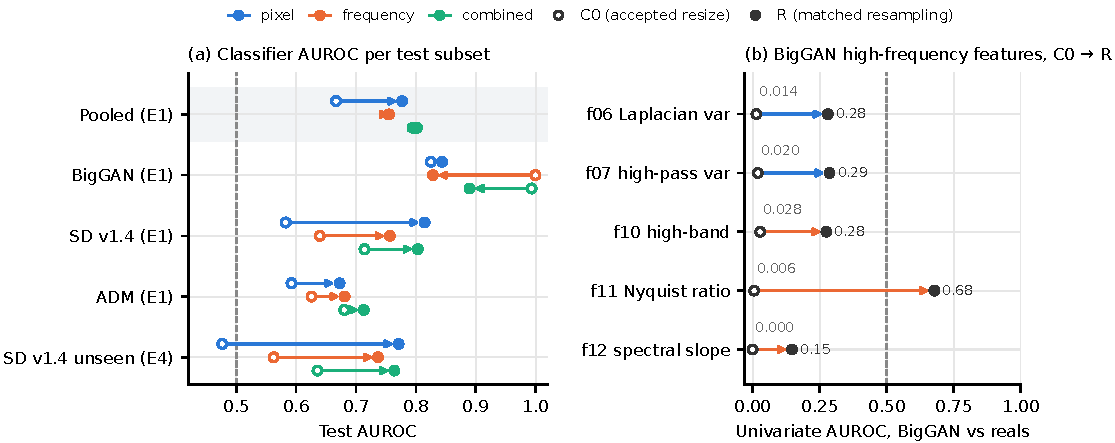
\includegraphics[width=\textwidth]{fig_resampling_swap.pdf}
\caption{Same pooled score, different story. (a) Test AUROC under the accepted resize (C0, open) and with every image given the same resampling history (R, filled), on the 599 test parents that survive the 128\,px crop. Pooled combined and frequency AUROC do not move; BigGAN falls, SD v1.4 rises, and on the unseen SD v1.4 (E4) the pixel arm goes from chance to 0.771. (b) Univariate AUROC of BigGAN vs.\ reals over all 2,994 surviving parents. The BigGAN images are pixel-identical in C0 and R, so the change comes from the reals now sharing BigGAN's upsampling. The near-perfect reversed separation largely disappears, the Nyquist ratio changes direction, and the spectral slope still separates.}
\label{fig:swap}
\end{figure*}

\begin{table}[t]
\centering
\caption{Accepted resize (C0) vs.\ resampling-matched (R), 599 test parents. $\Delta$ = R $-$ C0, paired bootstrap 95\% CI. Pixel and frequency: point AUROC C0 $\rightarrow$ R.}
\label{tab:swap}
\footnotesize
\setlength{\tabcolsep}{2.4pt}
\resizebox{\columnwidth}{!}{%
\begin{tabular}{@{}llccc@{}}
\toprule
Subset & Exp. & Combined $\Delta$ [95\% CI] & Pixel & Frequency \\
\midrule
Pooled & E1 & $+0.006$ [$-$0.036, 0.045] & 0.667$\rightarrow$0.777 & 0.755$\rightarrow$0.755 \\
BigGAN & E1 & $-0.104$ [$-$0.135, $-$0.070] & 0.825$\rightarrow$0.844 & 1.000$\rightarrow$0.828 \\
SD v1.4 & E1 & $+0.089$ [0.016, 0.161] & 0.583$\rightarrow$0.815 & 0.639$\rightarrow$0.757 \\
ADM & E1 & $+0.032$ [$-$0.030, 0.092] & 0.592$\rightarrow$0.673 & 0.626$\rightarrow$0.681 \\
SD v1.4 (unseen) & E4 & $+0.128$ [0.040, 0.208] & 0.477$\rightarrow$0.771 & 0.562$\rightarrow$0.737 \\
\bottomrule
\end{tabular}}
\end{table}

\subsection{Resampling-matched diagnostic}
Fig.~\ref{fig:swap} and Table~\ref{tab:swap} give the result. Giving every image the same resampling history leaves pooled AUROC unchanged for the combined arm (0.796 vs.\ 0.802, $\Delta = +0.006$ [$-0.036$, 0.045]) and for the frequency arm (0.755 in both), yet the per-generator picture changes. BigGAN, with unchanged pixels, drops from 1.000 to 0.828 in the frequency arm ($-0.172$ [$-0.225$, $-0.125$]). SD v1.4 rises in every arm, most for the pixel arm ($+0.232$ [0.162, 0.301]). On the unseen SD v1.4 (E4), the pixel arm goes from 0.477 to 0.771 ($+0.295$ [0.235, 0.358]). The ranking of the feature families changes with it: the paired pixel-minus-frequency difference is $-0.088$ [$-0.130$, $-0.045$] under C0 and $+0.022$ [$-0.015$, 0.056] under R, so the frequency arm's advantage is specific to the accepted resize. The combined arm stays best pooled under both (combined minus frequency $+0.047$ [0.026, 0.068] under R).

BigGAN remains separable under R (combined 0.890). The spectral slope still separates it (univariate 0.147), so the 2$\times$ upsampling explains the \emph{near-perfect} BigGAN result but not all of it. For SD v1.4, R removes the pipeline's $0.5\times$ downsampling, which averages away the finest scale of the native pixel grid, but it also narrows the field of view, so we do not attribute the SD rise to resampling alone.

\begin{figure}[t]
\centering
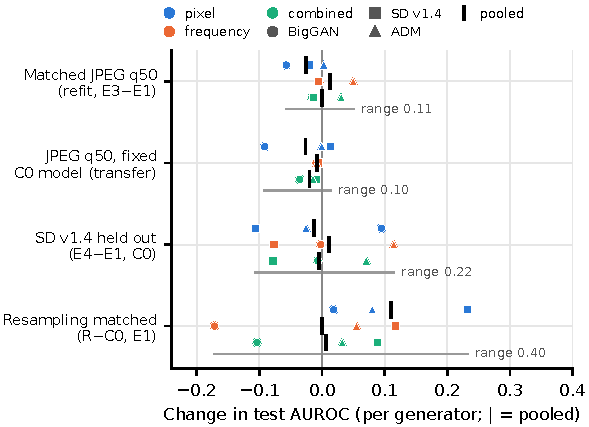
\includegraphics[width=\columnwidth]{fig_effect_sizes.pdf}
\caption{How far each manipulation moves AUROC. Each point is one arm (colour) on one generator (marker); the black tick is the pooled change. JPEG changes, refit or fixed-model, stay within about $\pm0.1$; holding SD v1.4 out moves per-generator AUROC over a range of 0.22; the resampling change moves it over 0.40 while the pooled combined AUROC stays near zero.}
\label{fig:effects}
\end{figure}

Fig.~\ref{fig:effects} puts the manipulations side by side. Across arms and generators, matched JPEG (refit or not) moves AUROC over a range of about 0.1, holding one generator out over 0.22, and the resampling change over 0.40, while its pooled effect on the combined arm is near zero.

\section{Discussion}

\textbf{What the features detect.} On this data, the strongest ``frequency evidence'' is the pipeline's own upsampling of one generator's output, and changing only the resampling step changes which generator looks easy and which feature family looks best, without changing the pooled score. Earlier work tied spectral artifacts to upsampling inside the generator~\cite{frank2020leveraging,durall2020watch,zhang2019artifacts}. Our result is a caution in the other direction: a shared, apparently fair preprocessing step can create or erase exactly the traces a spectral evaluation rewards. This agrees with the detector-level findings of~\cite{grommelt2024fake,guillaro2025bfree,zhou2026fragile} and makes them concrete for named statistics.

\textbf{Practical rule.} Evaluations of simple features should report per-generator results, record each class's native size and resampling factor, and state the resampling policy as part of the method. A pooled AUROC alone could not have revealed any of the effects in Fig.~\ref{fig:swap}.

\textbf{Compression.} Matched JPEG is mild for ranking (AUROC) but not for decisions. The fixed pixel model's false-positive rate on reals rises from 33\% to 52\% at q50, so a detector deployed at a clean-data threshold would drift even though AUROC barely moves.

\section{Limitations and Future Work}

The claims cover one dataset (GenImage validation folders, streamed from a mirror), three generator families, one JPEG encoder at three qualities, one held-out generator, and one random split, so intervals reflect test-set sampling only. Reals and fakes are not content-matched, so part of any separation may be content~\cite{gye2025sfld}. The resampling-matched condition R was designed after the main results were known and is reported as exploratory; for the diffusion families it changes the field of view as well as resampling. Future work: a pre-specified native-resolution protocol with a matched field of view, rotating the held-out generator, content-matched data, and a second JPEG encoder.

\section{Conclusion}

Under a pipeline fixed in advance, with matched processing, group splits, and explicit controls, the combined pixel and frequency set gave the highest pooled AUROC in every setting (0.793 clean; 0.629 on an unseen diffusion generator under JPEG~75), matched compression changed pooled AUROC by at most 0.027, and generator shift cost about 0.08. The controls then showed that the pooled scores hide the main effect: the dataset's processing history, and the pipeline's own resampling of it, decide which generator is easy and whether pixel or frequency statistics look stronger. For simple features, the resampling history is part of the result and must be reported with it.

\bibliographystyle{IEEEtran}
\bibliography{refs}

\end{document}
